\chapter{Estado de la cuestión}
\label{chap:estado_cuestion}

Aquí debo hablar de todo lo relacionado con mi objeto de estudio, y su estado del arte, no tanto meter teoría, que se supone ya en marco teórico.

Quiero ser breve e ir al grano (tampoco hay mucho que poner aquí, ya que está poco o nada estudiado). Si algo hay que explicarlo más, mejor en marco teórico...


\begin{itemize}
    \item Modelos de IA generativa aplicados a la música.
    \item LLM asistentes para la creación de código de programación.
    \item Lenguajes de programación musical.
    \item Prompting engineering.
    \item LLM y música (MIDI y otras representaciones).
    \item LLM y música con lenguajes de programación.
\end{itemize}

\section{Modelos de IA generativa aplicados a la música}
    Repasar especialmente los últimos modelos lanzados por Google y Amazon\dots y su estado.

\section{LLM asistentes para la creación de código de programación}
\label{sec:llm_asistentes_creacion_codigo_programacion}
    GPT-4 como estado del arte. Software específico como Github Copilot. Hablar de los más importantes LLM y su rendimiento en la programación.


    \begin{figure}[h]
        \caption{Relación AI, ML y DL}
        \centering
        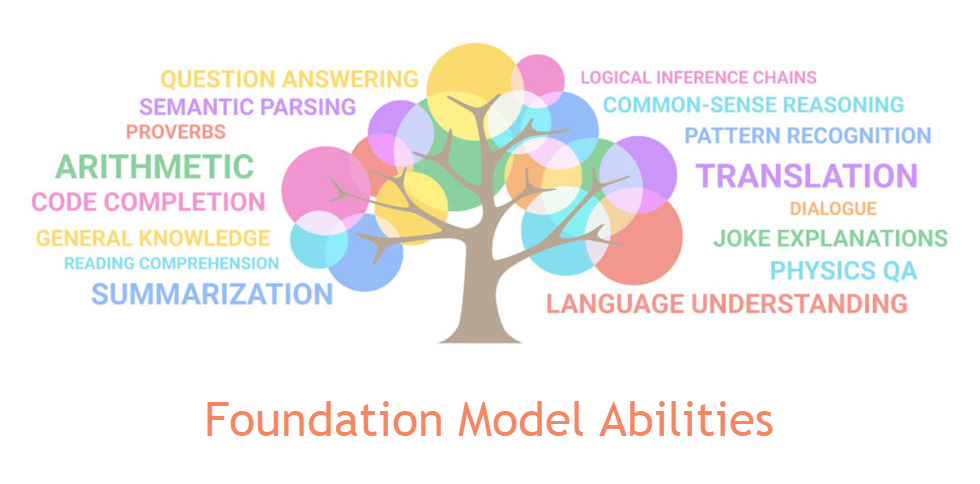
\includegraphics[width=0.8\textwidth]{./figuras/fundation_models_habilities.png}
        \source{\cite{GPT3RiseFoundation}}
        \label{fig:fundation_models_habilities}
    \end{figure}

\section{Lenguajes de programación musical}
    Lenguajes a modo de código de programación, como Overtone, Pure Data, Sonic Pi, Supercollider, Max MSP. Representaciones musicales susceptibles de ser generadas por LLM, como el MIDI, MusicXML, ABC, Lilypond, etc.

\section{Prompting engineering. Estado del arte}
    Un repaso por los papers más significativos y actuales sobre esta cuestión, especialmente las que implican la generación de código.

\section{\textit{Retrieval-Augmented Generation} (RAG)}
    Una de las técnicas más potentes para la generación de código, que combina la recuperación de información con la generación de texto. También de OpenAI Assistant, que ha presentado en el Keynote de 2023. \cite{WhatRetrievalaugmentedGeneration2021} y \cite{lewisRetrievalAugmentedGenerationKnowledgeIntensive2021}

\section{LLM y música (MIDI y otras representaciones) y el problema del significado}
    Quiero exponer la distancia que supone conocer un lenguaje y usarlo para crear arte con él. Que un sistema (o un ser humano) conozca la sintaxis de un lenguaje no significa que pueda crear con él obras de arte... al menos si no se le entrena con suficientes datos.
    
    Usar como bibliografía: el paper \cite{lewisRetrievalAugmentedGenerationKnowledgeIntensive2021} y la web \cite{WhatRetrievalaugmentedGeneration2021}

\section{LLM y música en SuperCollider}